% !TeX root = main.tex
% !TeX spellcheck = en-US
% !TeX encoding = utf8


\chapter{Results and Evaluation}
\label{chap:results}

All experiments and analyses were performed as previously explained in \cref{chap:testing,chap:analysis}.

\section{Part I - Choosing the Optimization Algorithm}
\label{chap:part1}

\subsection{Convergence Behavior}

\begin{figure}[h]
	\centering
	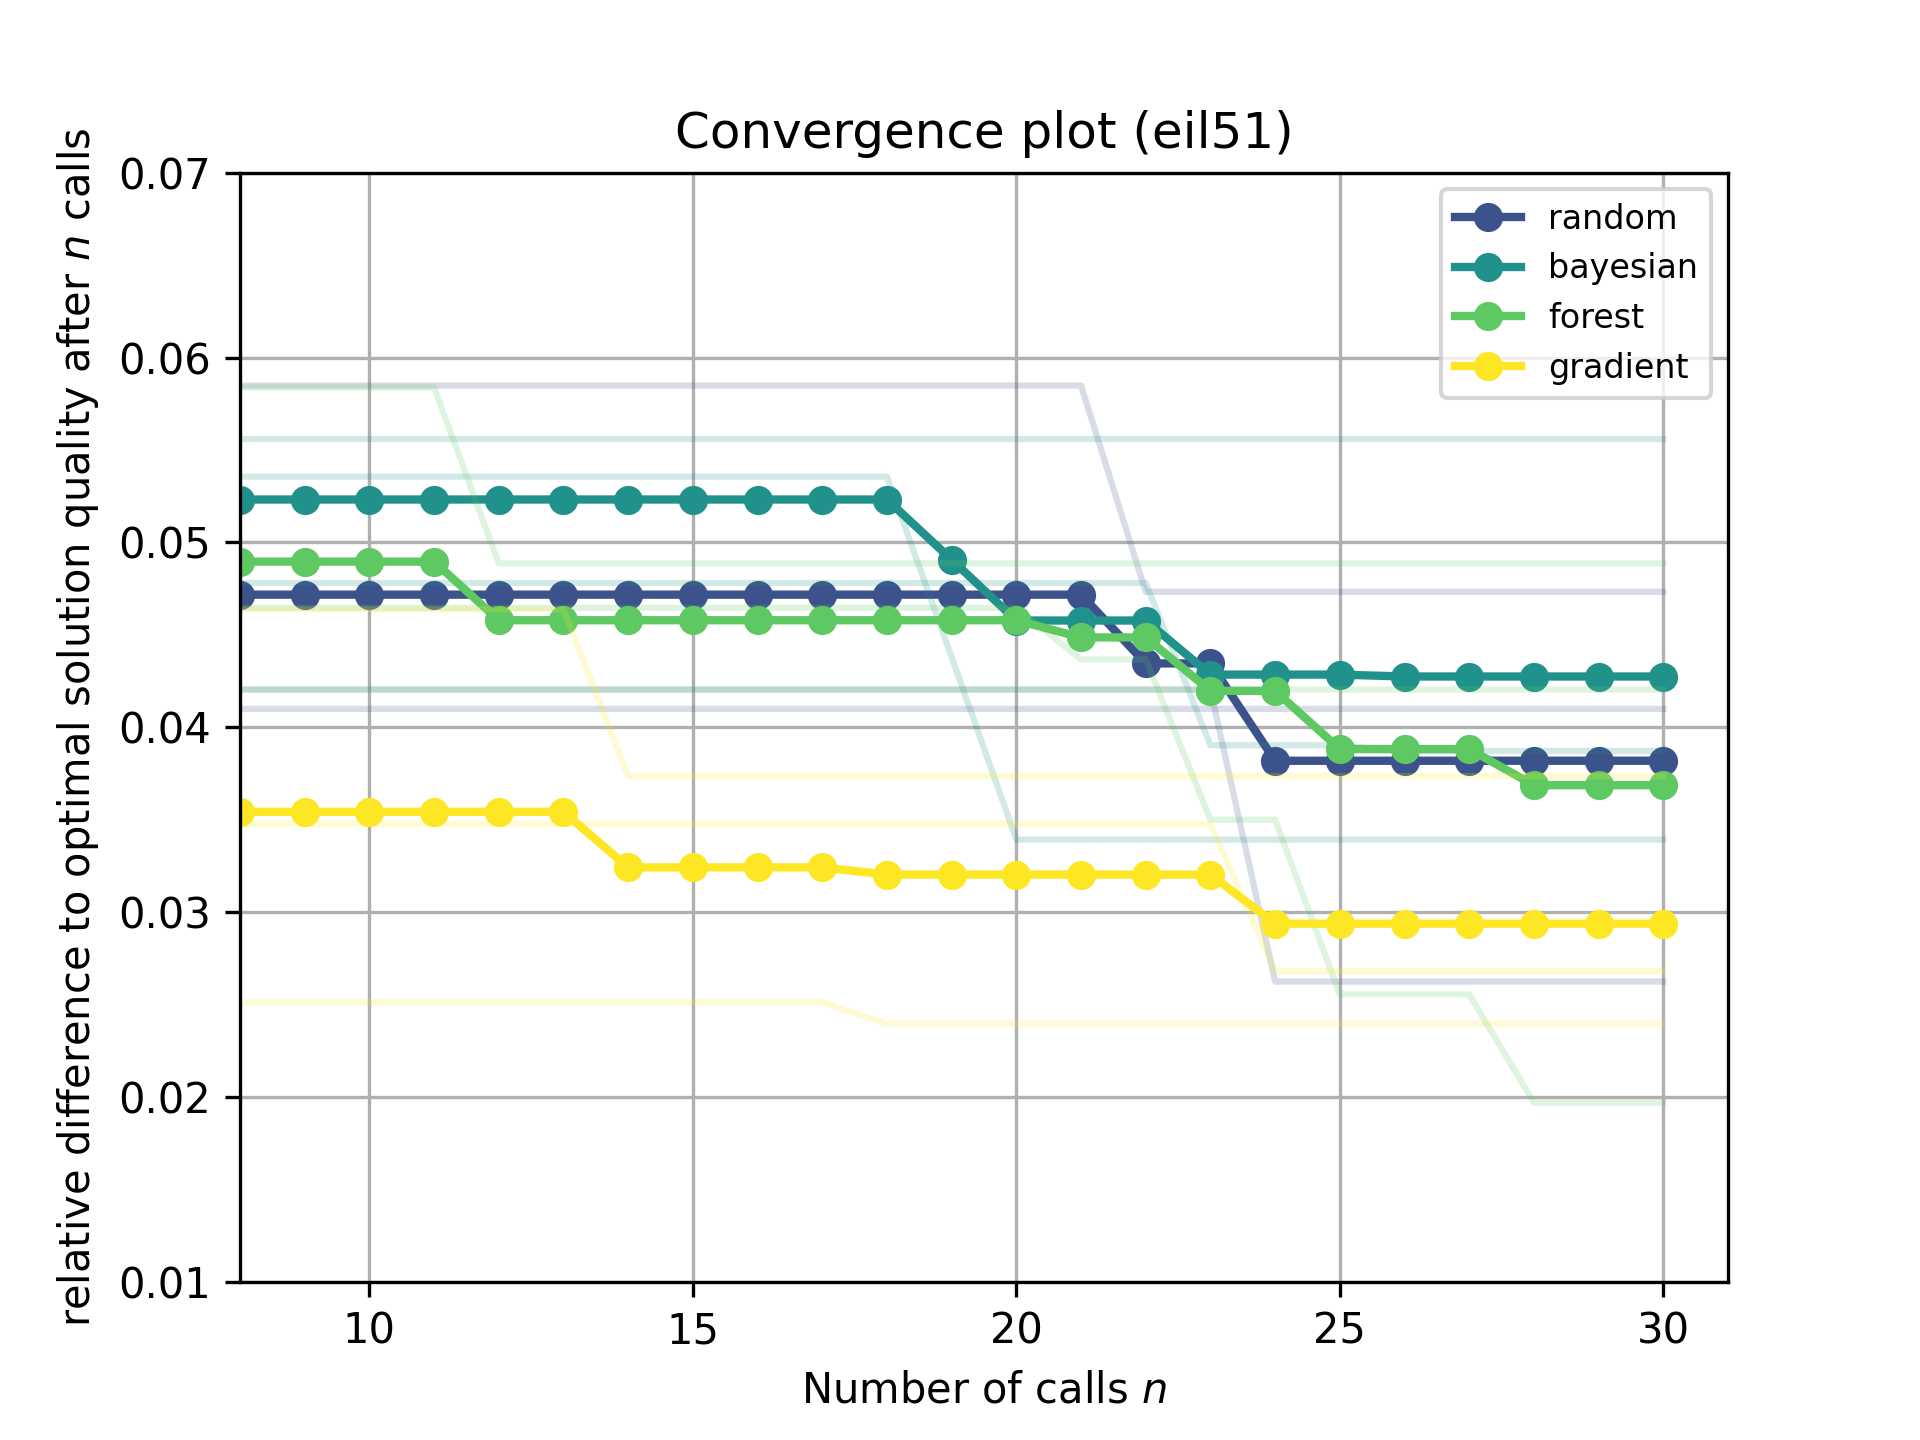
\includegraphics[width=0.75\textwidth]{results/part1/convergence_eil51.png}
	\caption{Text}
	\label{fig:convergence_eil51}
\end{figure}

\begin{figure}[h]
	\centering
	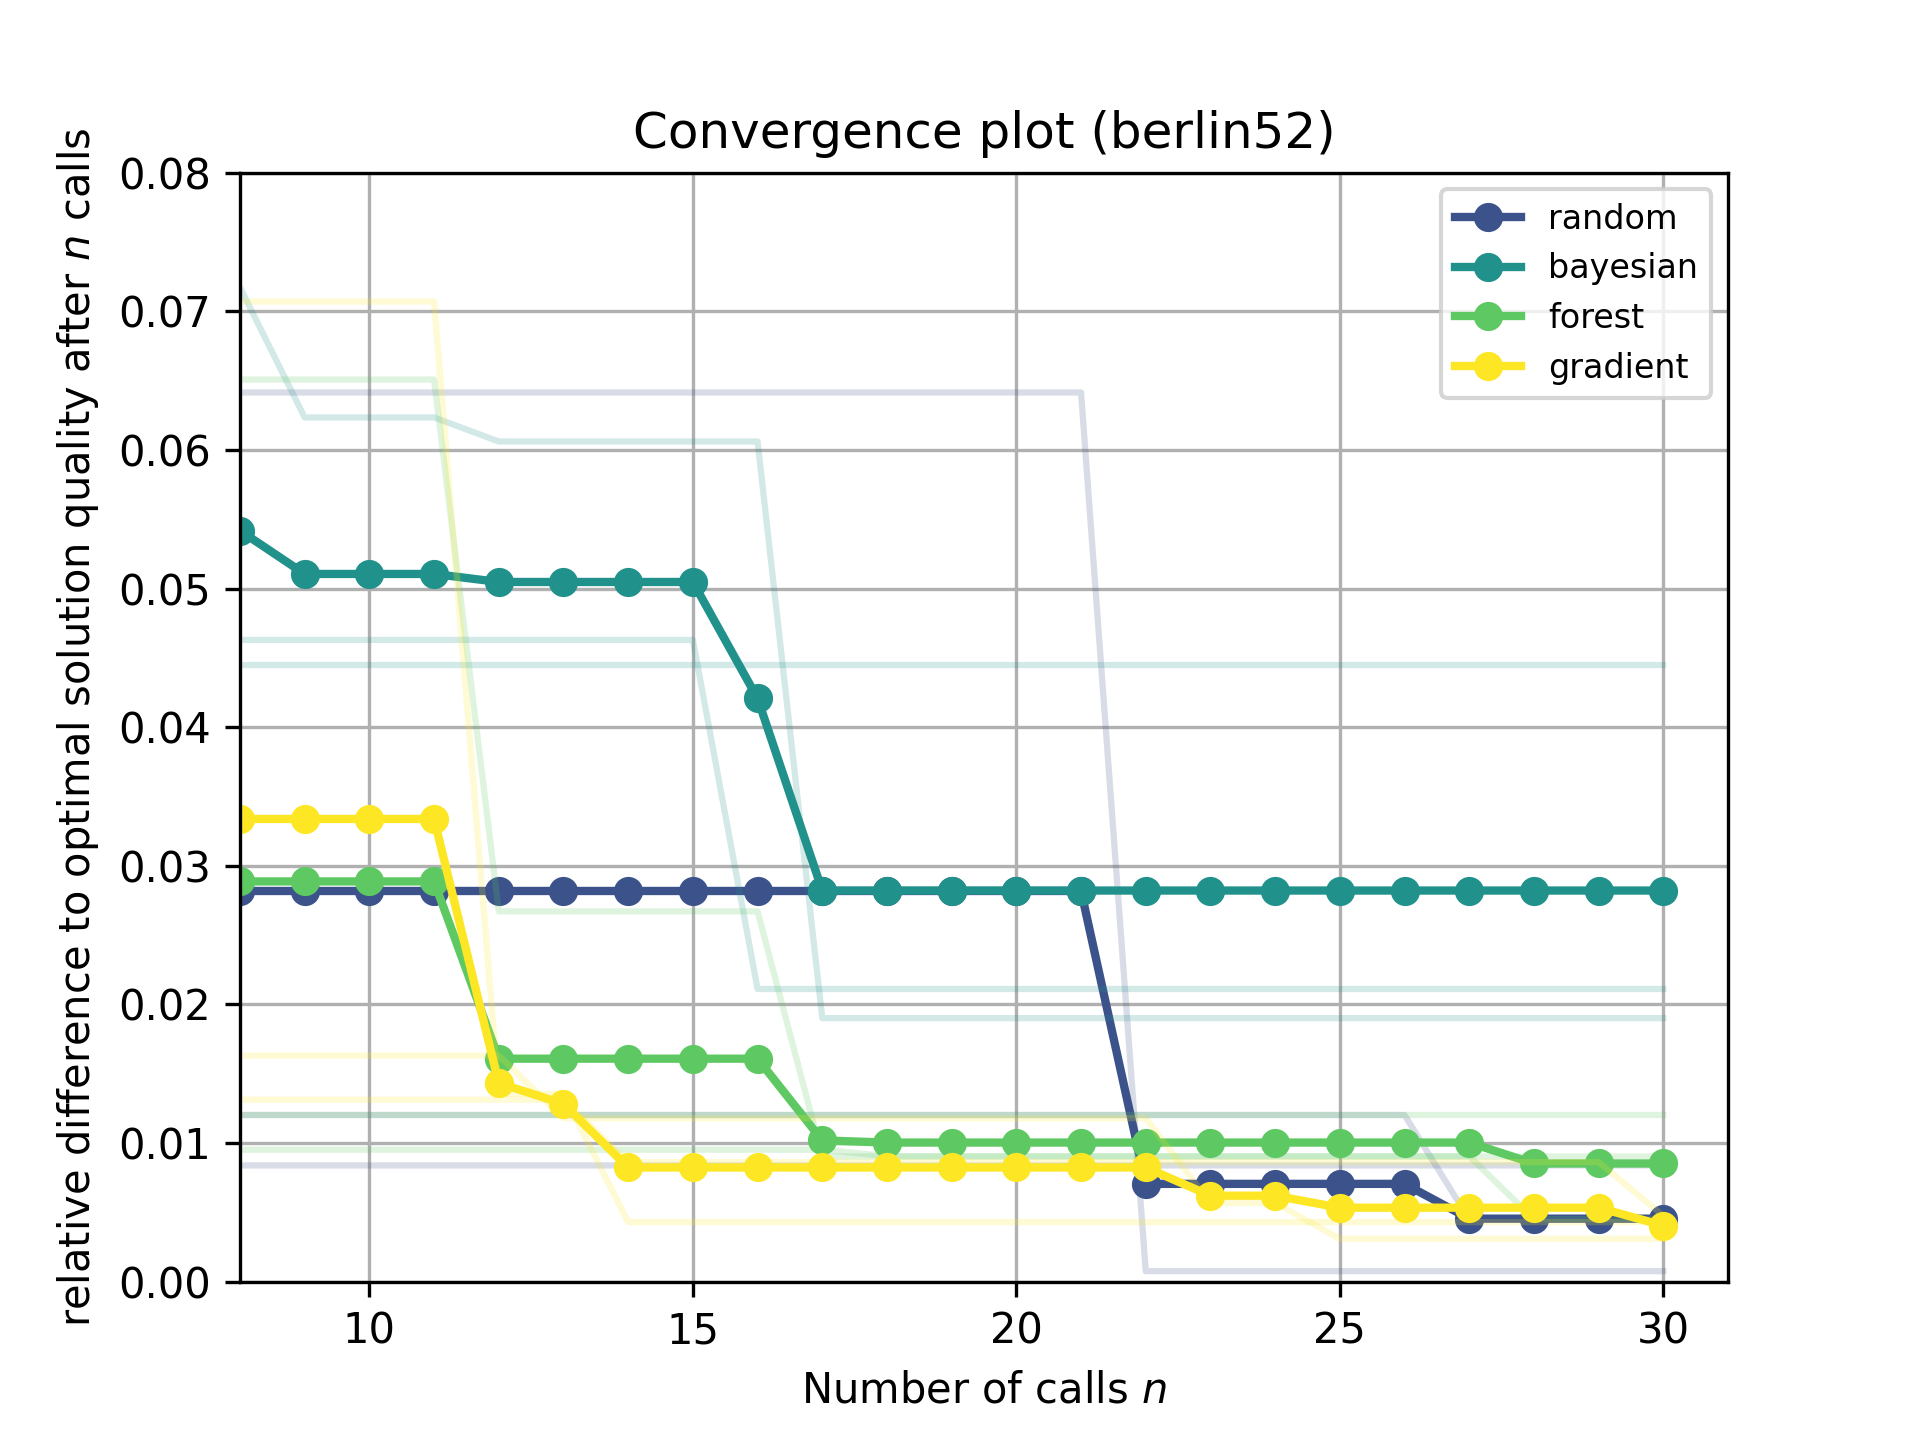
\includegraphics[width=0.75\textwidth]{results/part1/convergence_berlin52.png}
	\caption{Text}
	\label{fig:convergence_berlin52}
\end{figure}

\begin{figure}[h]
	\centering
	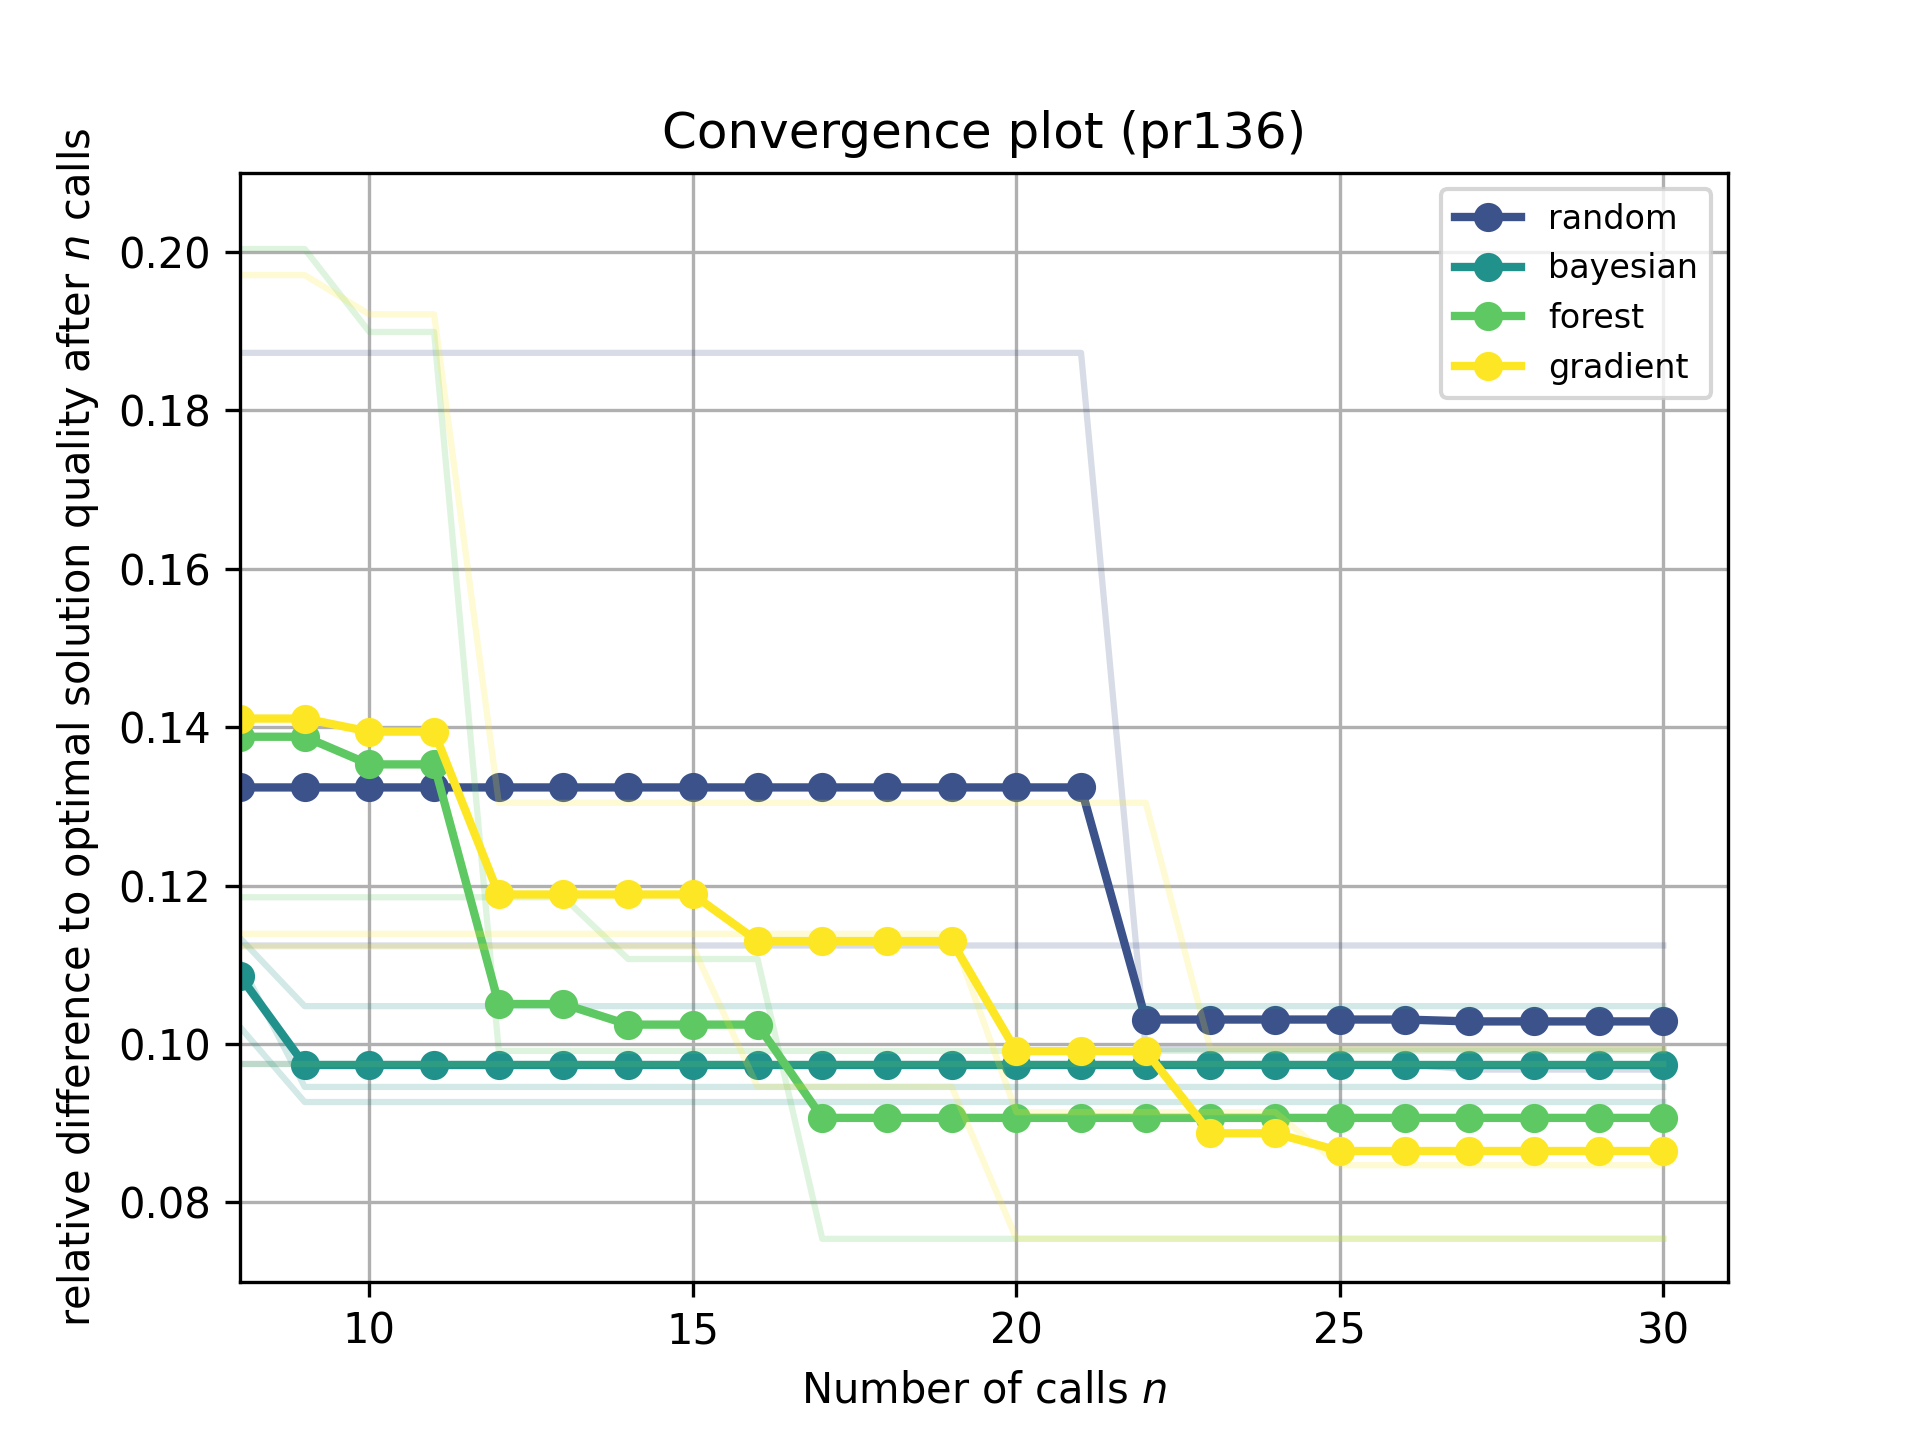
\includegraphics[width=0.75\textwidth]{results/part1/convergence_pr136.png}
	\caption{Text}
	\label{fig:convergence_pr136}
\end{figure}

\begin{figure}[h]
	\centering
	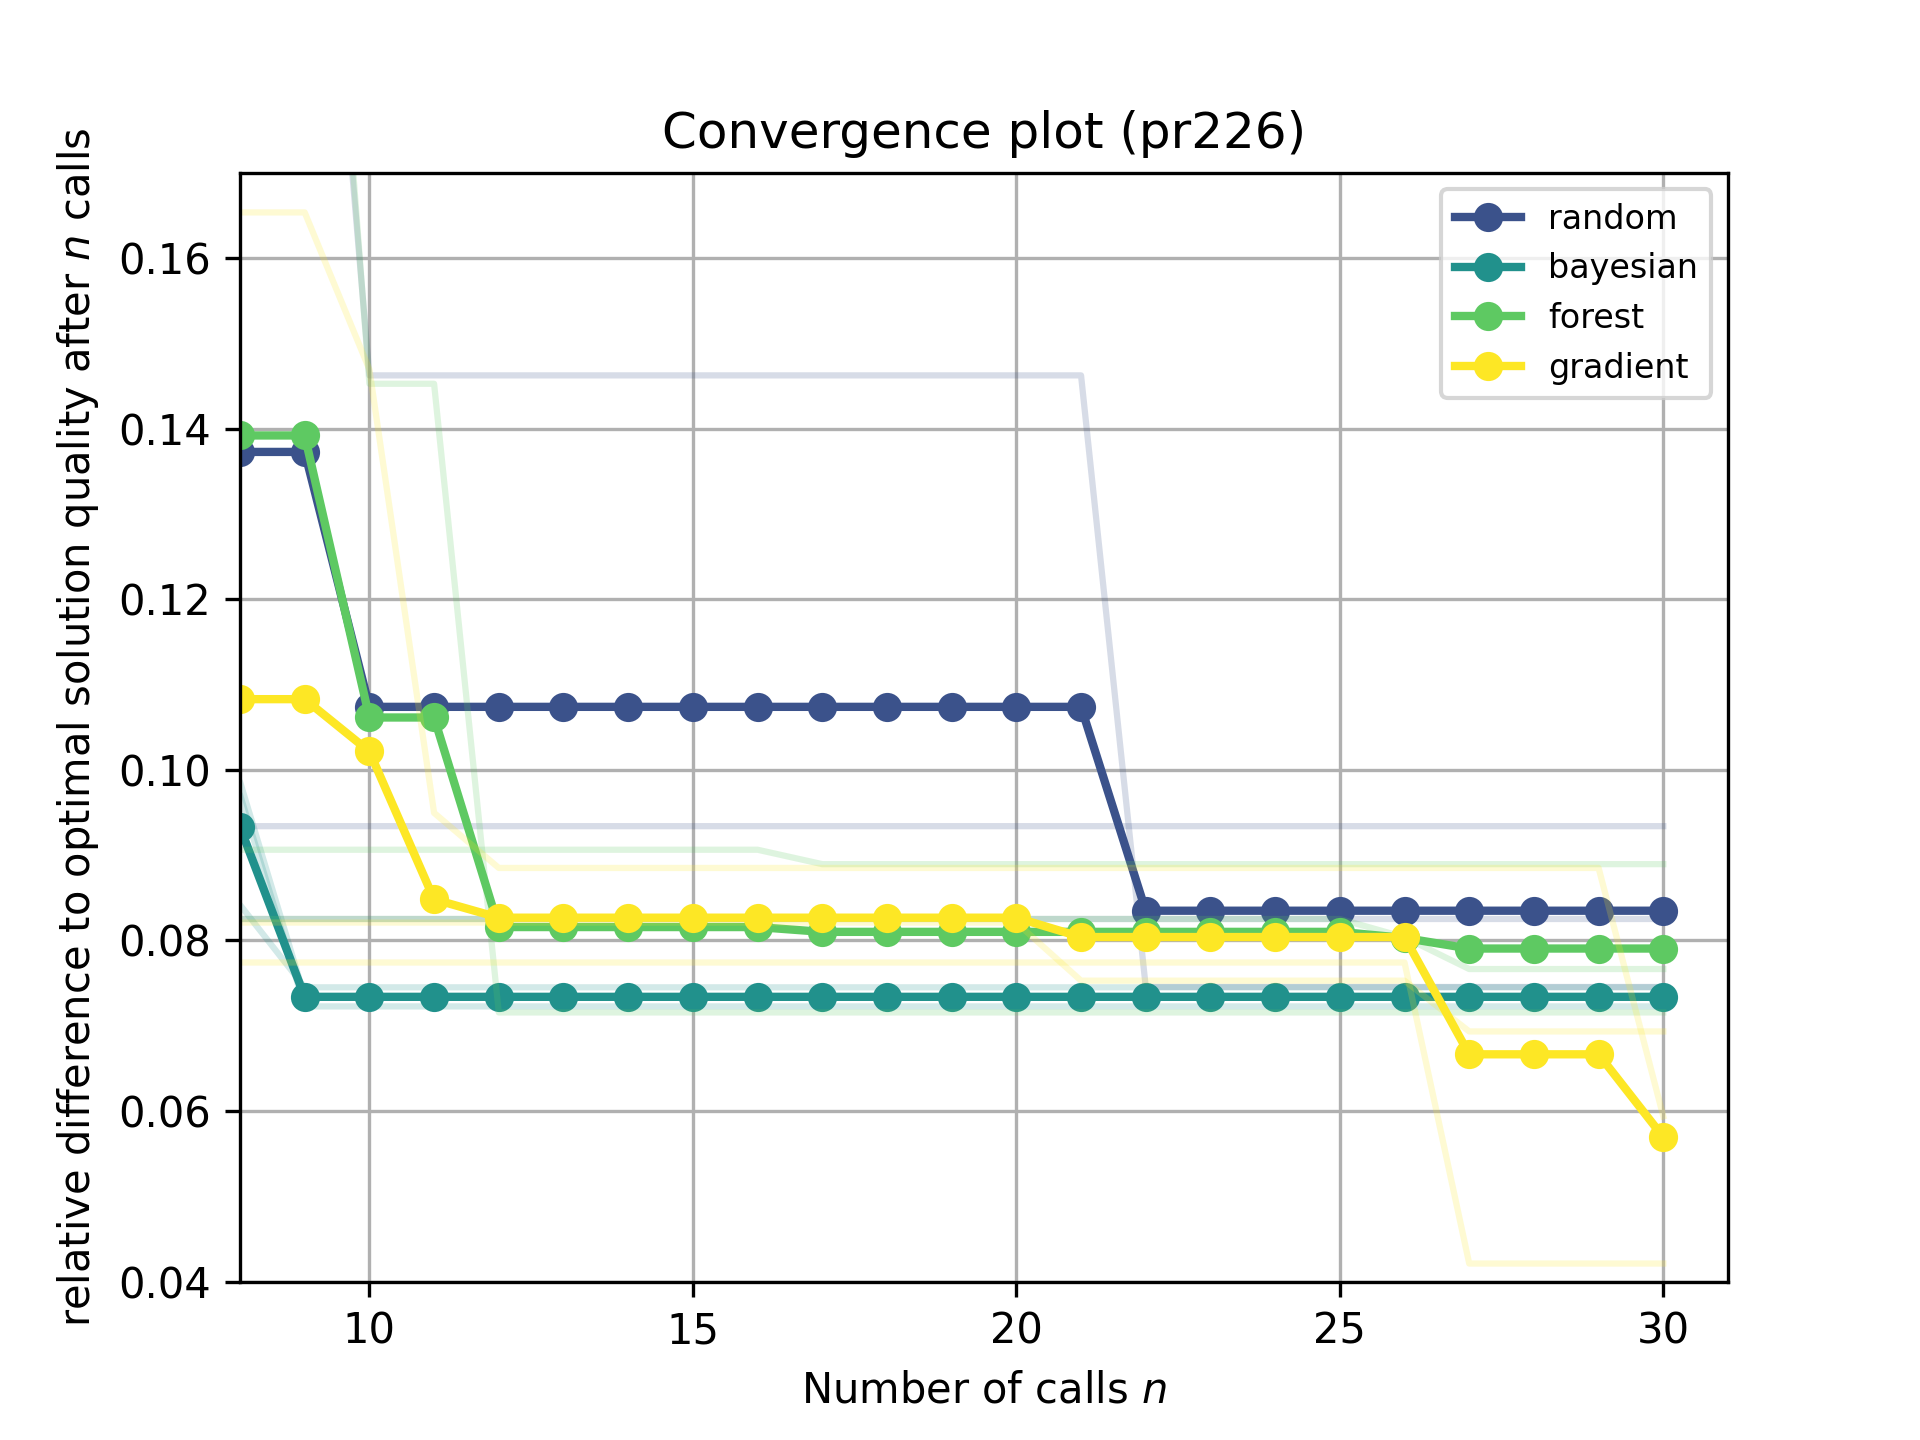
\includegraphics[width=0.75\textwidth]{results/part1/convergence_pr226.png}
	\caption{Text}
	\label{fig:convergence_pr226}
\end{figure}

\begin{figure}[h]
	\centering
	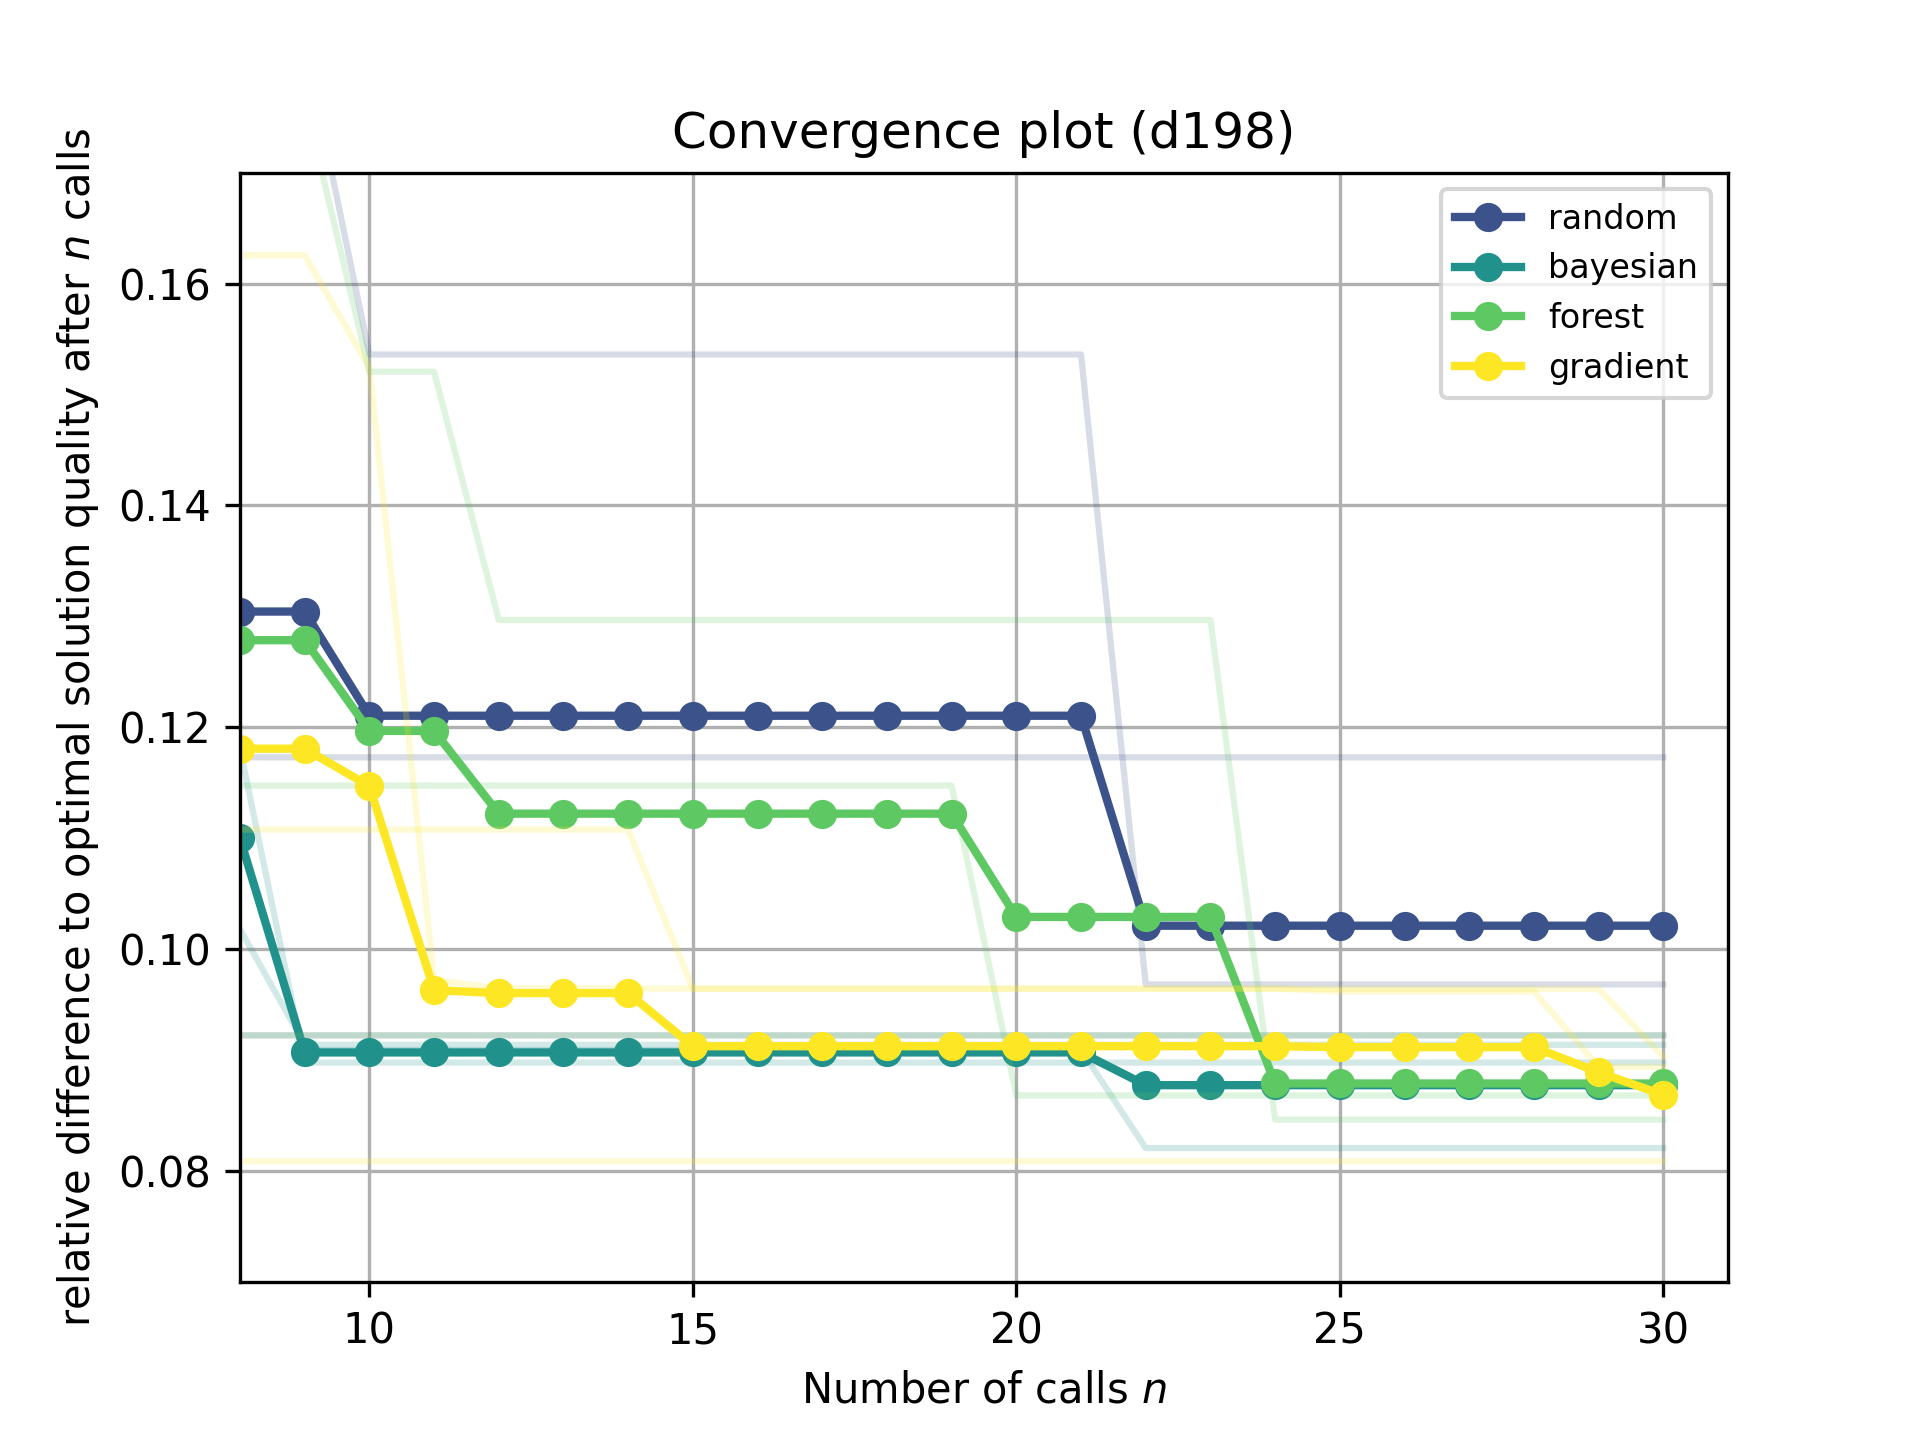
\includegraphics[width=0.75\textwidth]{results/part1/convergence_d198.png}
	\caption{Text}
	\label{fig:convergence_d198}
\end{figure}

\begin{figure}[h]
	\centering
	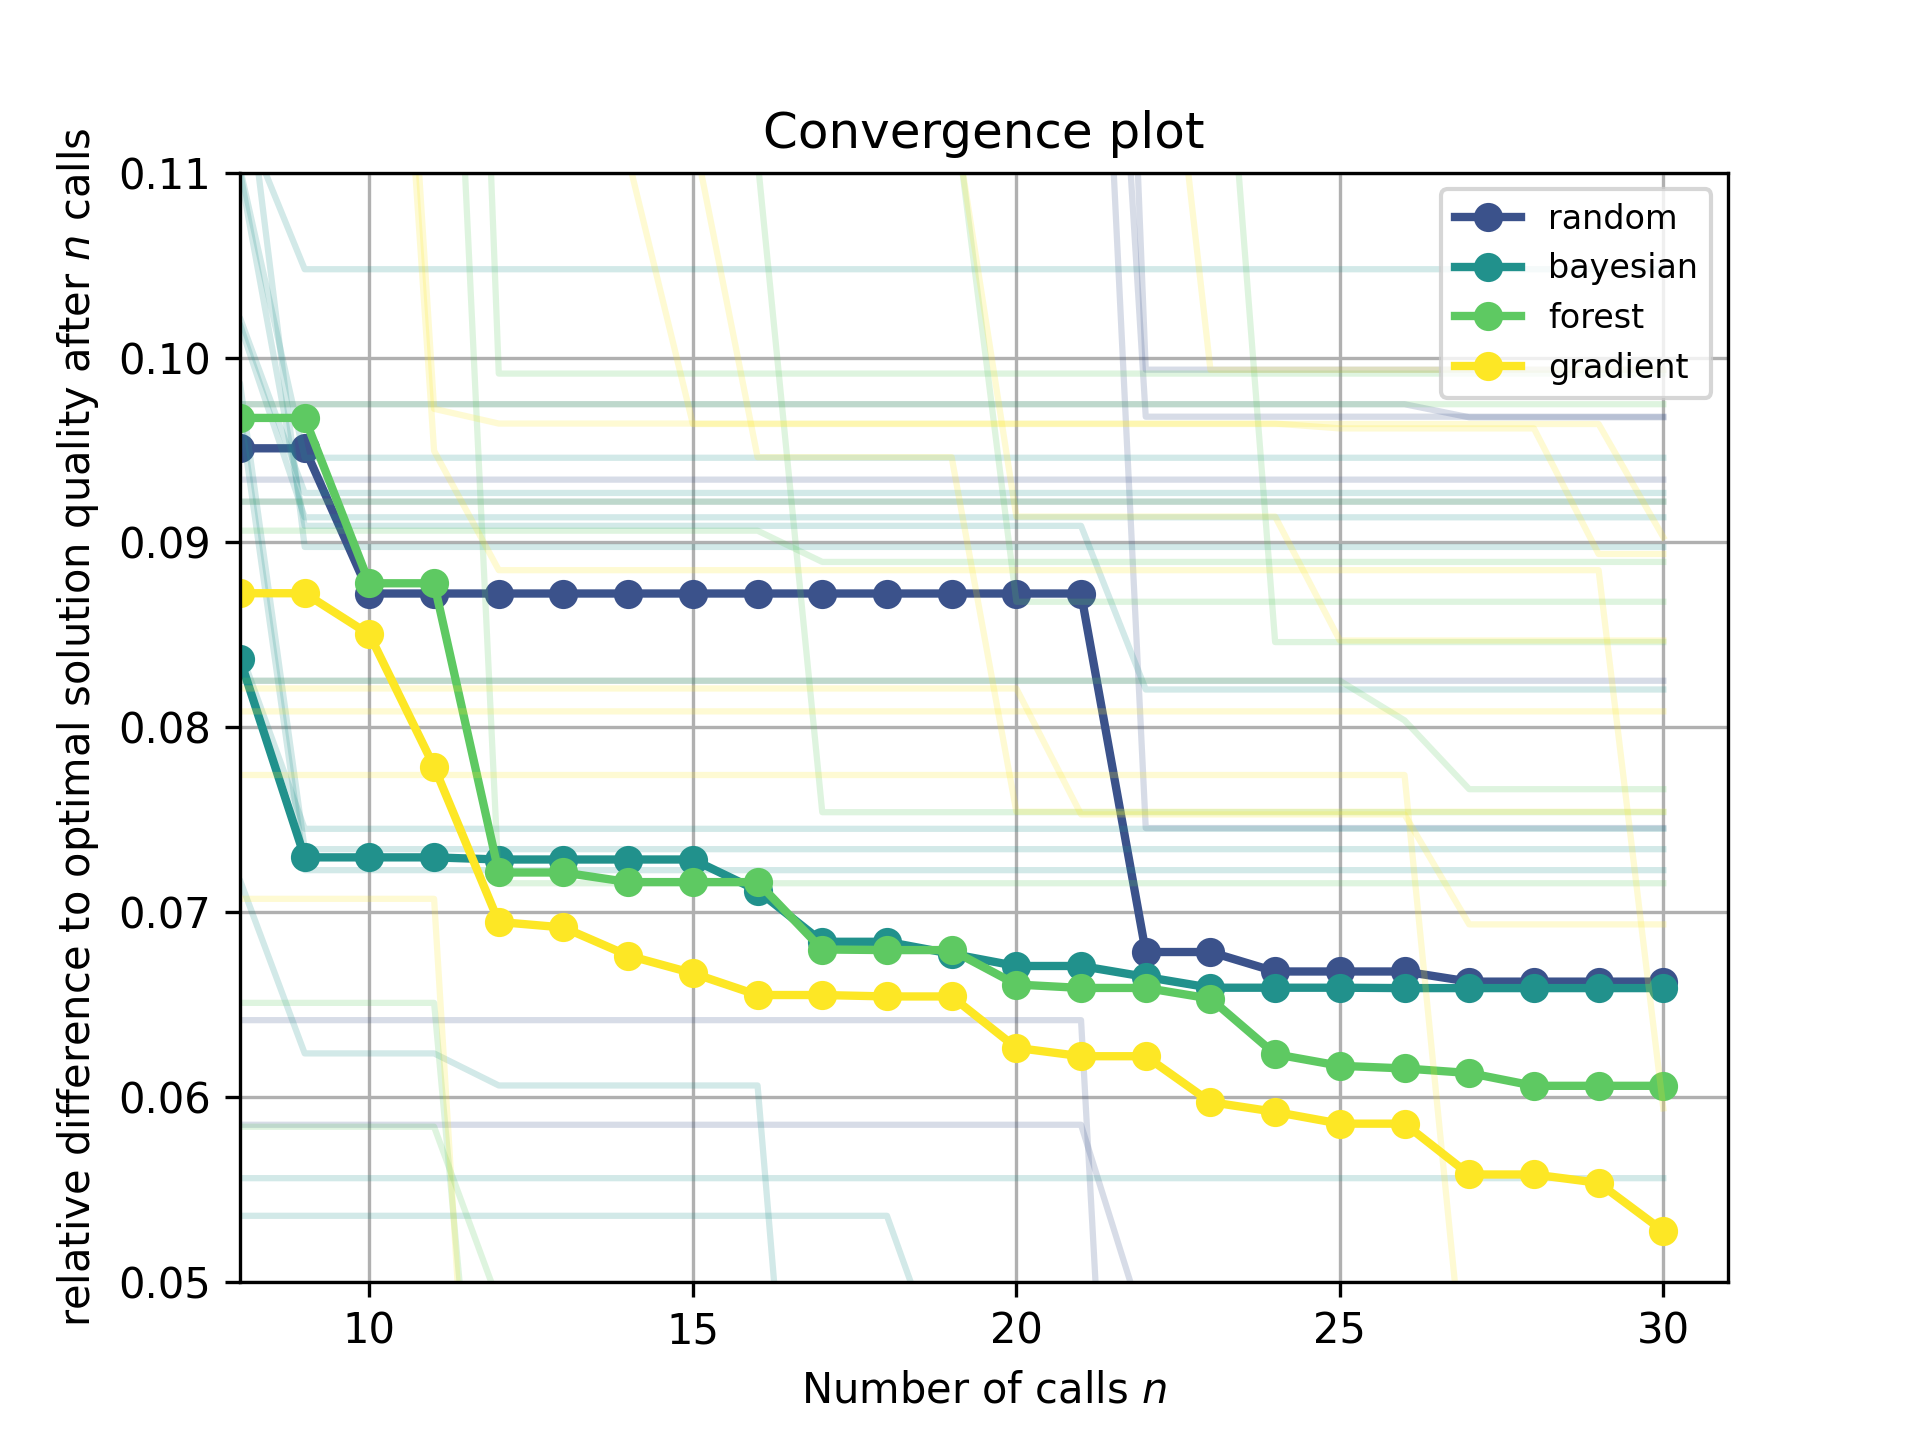
\includegraphics[width=0.75\textwidth]{results/part1/convergence_all.png}
	\caption{Text}
	\label{fig:convergence_all}
\end{figure}


\begin{figure}[h]
	\centering
	\begin{subfigure}{0.495\textwidth}
		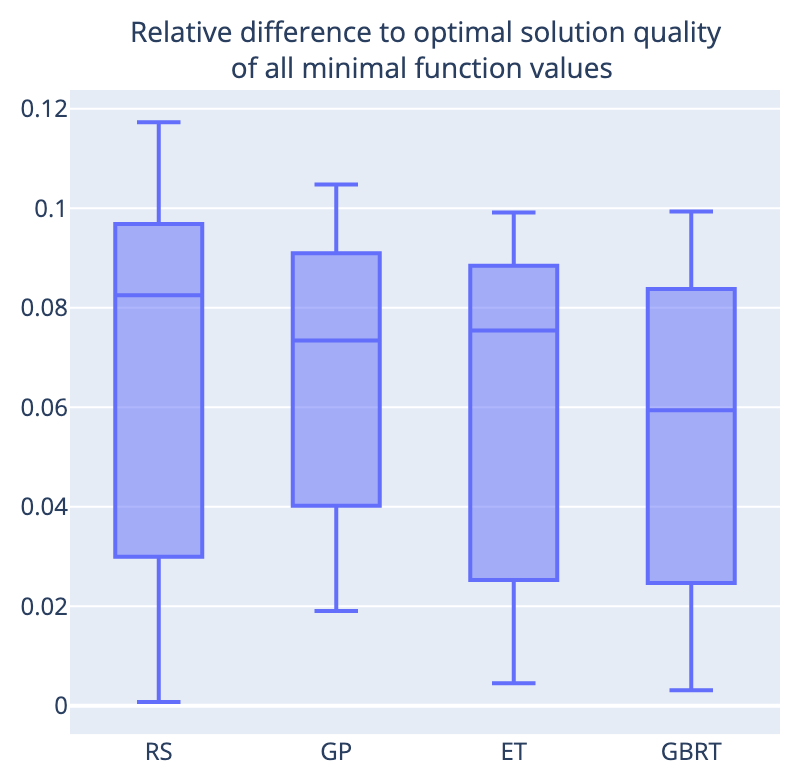
\includegraphics[width=\textwidth]{results/part1/convergence_stats_boxplot_1.png}
		\caption{Text}
		\label{fig:convergence_stats_boxplot_1}
	\end{subfigure}
	\begin{subfigure}{0.495\textwidth}
		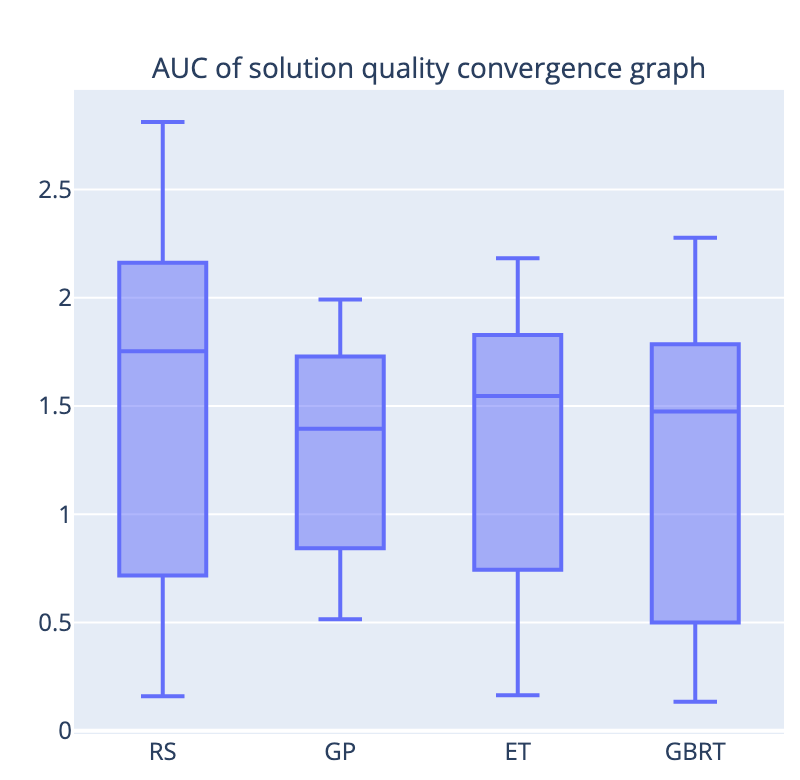
\includegraphics[width=\textwidth]{results/part1/convergence_stats_boxplot_2.png}
		\caption{Text}
		\label{fig:convergence_stats_boxplot_2}
	\end{subfigure}
	\caption{Text}
	\label{fig:convergence_stats_boxplots}
\end{figure}

\begin{table}[h]
	\centering
	\caption[The \gls{auc} and minimal $RPD$ value of all optimization runs]{The \gls{auc} and minimal $RPD$ value of all optimization runs for each method and instance, and for the mean over all instances.}
	\label{tab:part1-stats}
	\begin{adjustbox}{width=1\textwidth}
	\begin{tabular}{l !{\vrule width 1pt} l|l !{\vrule width 1pt} l|l !{\vrule width 1pt} l|l !{\vrule width 1pt} l|l !{\vrule width 1pt} l|l !{\vrule width 1pt} l|l}
		~ & \multicolumn{2}{c !{\vrule width 1pt}}{eil51} &  \multicolumn{2}{c !{\vrule width 1pt}}{berlin52} &  \multicolumn{2}{c !{\vrule width 1pt}}{pr136} & \multicolumn{2}{c !{\vrule width 1pt}}{pr226} & \multicolumn{2}{c !{\vrule width 1pt}}{d198} & \multicolumn{2}{c}{mean}\\ \hline
		~ & \gls{auc} & min & \gls{auc} & min & \gls{auc} & min & \gls{auc} & min & \gls{auc} & min & \gls{auc} & min \\ \noalign{\hrule height 1pt}
		RS & 0.830 & 0.026 & 0.347 & 0.001  & 2.266 & 0.097 & 1.837 & 0.075 & 2.139 & 0.092 & 1.484 & 0.058\\ \hline
		GP & 0.900 & 0.034 & 0.650 & 0.019 & 1.850 & 0.093 & 1.394 & 0.072 & 1.698 & 0.082 & 1.298 & 0.060\\ \hline
		ET & 0.819 & 0.020 & 0.227 & 0.005 & 1.809 & 0.075 & 1.547 & 0.072 & 1.940 & 0.085 & 1.268 & 0.051\\ \hline
		GBRT & 0.601 & 0.024 & 0.159 & 0.003 & 1.948 & 0.075 & 1.497 & 0.042 & 1.745 & 0.081 & 1.190 & 0.045\\ 
	\end{tabular}
\end{adjustbox}
\end{table}



\subsection{Statistical Tests}

\begin{table}[h]
	\centering
	\caption{Text}
	\label{tab:kruskal-test}
	\begin{tabular}{l|l|l|l|l|l}
		~ & eil51 & berlin52 & pr136 & pr226 & d198 \\ \hline
		statistic & 47.893 &	46.960&	29.898	&57.998	&46.514 \\
		$p$-value & \num{2.244e-10} & \num{3.544e-10} &\num{1.450e-6} & \num{1.574e-12} & \num{4.410e-10} \\
	\end{tabular}
\end{table}

\begin{table}[h]
	\centering
	\caption{Text}
	\label{tab:conover-p}
	
	\begin{adjustbox}{width=1\textwidth}
		\begin{tabular}{ l | l | l | l | l | l | l}
			TSP & \gls{rs} vs. \gls{gp} & \gls{rs} vs. \gls{et} & \gls{rs} vs. \gls{gbrt} & \gls{gp} vs. \gls{et} & \gls{gp} vs. \gls{gbrt} & \gls{et} vs. \gls{gbrt} \\ \hline
			eil51 & \num{0.626022837} & \num{1} & \cellcolor{green!25} \num{1,3613E-11} & \cellcolor{green!25} \num{0,045498418} &  \cellcolor{green!25} \num{9,87937E-15} &\cellcolor{green!25}  \num{1,71033E-09} \\ \hline
			berlin52 & \cellcolor{green!25} \num{6,31757E-10} & \num{1} & \num{0,055983678} & \cellcolor{green!25} \num{4,84375E-08} & \cellcolor{green!25} \num{5,09448E-15} & \cellcolor{green!25} \num{0,002694824} \\ \hline
			pr136 & \cellcolor{green!25} \num{4,40687E-06} &\cellcolor{green!25}  \num{1,47269E-07} & \cellcolor{green!25} \num{1,49122E-04} & \num{1} & \num{1} & \num{0,524644367} \\ \hline
			pr226 & \cellcolor{green!25} \num{1,07734E-22} & \cellcolor{green!25} \num{1,85077E-10} & \cellcolor{green!25} \num{1,83947E-11} & \cellcolor{green!25} \num{2,22893E-08} & \cellcolor{green!25} \num{2,06853E-07} & \num{1} \\ \hline
			d198 & \cellcolor{green!25} \num{4,0384E-15} & \cellcolor{green!25} \num{0,001090407} & \cellcolor{green!25} \num{2,6556E-07} & \cellcolor{green!25} \num{1,20061E-07} & \cellcolor{green!25}  \num{0,000563675} & \num{0,210301266} \\
		\end{tabular}
	\end{adjustbox}
\end{table}

\begin{table}[h]
	\centering
	\caption{Text}
	\label{tab:conover-t}
	
	\begin{adjustbox}{width=1\textwidth}
	\begin{tabular}{ l | l | l | l | l | l | l}
		TSP & \gls{rs} vs. \gls{gp} & \gls{rs} vs. \gls{et} & \gls{rs} vs. \gls{gbrt} & \gls{gp} vs. \gls{et} & \gls{gp} vs. \gls{gbrt} & \gls{et} vs. \gls{gbrt} \\ \hline
		eil51 & \num{-1,643854208} & \num{1,099460932} & \cellcolor{green!25} \num{8,358037955} & \cellcolor{green!25} \num{2,74331514} & \cellcolor{green!25} \num{10,00189216} & \cellcolor{green!25} \num{7,258577024} \\ \hline
		berlin52 & \cellcolor{green!25} \num{-7,486334021} & \num{-1,00169258} & \num{2,667665503} & \cellcolor{green!25} \num{6,484641441} & \cellcolor{green!25} \num{10,15399952} & \cellcolor{green!25} \num{3,669358084} \\ \hline
		pr136 & \cellcolor{green!25} \num{5,39986544} & \cellcolor{green!25} \num{6,222702079} & \cellcolor{green!25} \num{4,491316652} & \num{0,822836638} & \num{-0,908548788} & \num{-1,731385427} \\ \hline
    	pr226 & \cellcolor{green!25} \num{14,43190942} & \cellcolor{green!25} \num{7,765991183} & \cellcolor{green!25} \num{8,289835445} & \cellcolor{green!25} \num{-6,665918233} & \cellcolor{green!25} \num{-6,142073971} & \num{0,523844262} \\ \hline
    	d198 & \cellcolor{green!25} \num{10,20744357} & \cellcolor{green!25} \num{3,936409009} & \cellcolor{green!25} \num{6,082589453} & \cellcolor{green!25} \num{-6,271034565} & \cellcolor{green!25} \num{-4,124854122} & \num{2,146180444} \\ \hline
	\end{tabular}
	\end{adjustbox}
\end{table}

\subsection{Conclusion}

\section{Part II - Choosing the Parameter Sets}
\label{chap:part2}

\subsection{Robustness of Parameter Values}

\subsection{Correspondence with Problem Instances}

\subsection{Parameter Importance}


\section{Part III - Evaluating the Parameter Sets}
